\chapter{\PLTL and \LTLf}\label{ch:theory}
This chapter will deal with the theoretical framework on which all topics present in the thesis are based. Initially, we will introduce the widely known Linear-Time Temporal Logic (\LTL) and the Past Linear Time Temporal Logic (\PLTL), focusing on their syntax and semantic. Secondly, we will talk about the concept of \textit{Finite Trace} in these formal languages and how it changes them. Specifically, we will describe the Linear Time Temporal Logic over Finite Traces (\LTLf). Then, we will illustrate the theory behind the transformation of an \LTLf or \PLTL formula to a Deterministic Finite State Automaton (\DFA). Finally, we will describe the translation of an \LTLf or \PLTL formula to the classic First-Order Logic formalism (\FOL) and the translation of a \FOL formula into a program that the \MONA, a tool that translates formulas into a \DFA, can manage. Some examples will be provided, but we will suppose the reader to be confident with classical logic and automata theory.
\section{Linear Temporal Logic (\LTL)}\label{sec:ltl-definition}
\textit{Temporal Logic} formalisms are a set of formal languages designed for representing temporal information and reasoning about time within a logical framework \citep{sep-logic-temporal}. Indeed, these logics are used when propositions have their truth value dependent on time.

In this scenario, we find the \textit{Linear Temporal Logic} (\LTL) which is a a very well known modal temporal logic with modalities referring to time. It was originally proposed in \citep{Pnueli:1977:TLP:1382431.1382534} as a specification language for concurrent programs. Consequently, \LTL has been extensively used in Artificial Intelligence and Computer Science. For instance, it has been employed in planning, reasoning about actions, declarative process mining and verification of software/hardware systems.
\subsection{Syntax}\label{ltl-syntax}
Given a set of propositional symbols $\P$, a valid \LTL formula $\varphi$ is defined as follows:
\[\begin{array}{rcl}
\varphi &::=& a \mid \lnot \varphi \mid \varphi_1\land \varphi_2 \mid \Next\varphi \mid \varphi_1 \lUntil \varphi_2
\end{array}
\]
where $a\in \P$. The unary operator \Next  (\emph{next-time}) and the binary operator $\lUntil$  (\emph{until}) are temporal operators and we use $\top$ and $\bot$ to denote $\true$ and $\false$ respectively. Moreover, all classical logic operators $\lOR, \Rightarrow, \Leftrightarrow, true$ and $false$ can be used. 
Intuitively, \Next $\varphi$ says that $\varphi$ is true at the \textit{next} instant, $\varphi_1 \lUntil \varphi_2$ says that at some future instant, $\varphi_2$ will hold and \textit{until} that point $\varphi_1$ holds. We also define common abbreviations for some specific temporal formulas: \emph{eventually} as $\Diamond \varphi \doteq \true \lUntil \varphi$, \emph{always} as $\Box \varphi \doteq \lnot \Diamond \lnot \varphi$, \emph{weak-next} as $\Wnext \varphi \doteq \lnot \Next \lnot \varphi$ and \emph{release} as $\varphi_1 \Release \varphi_2 \doteq \lnot (\lnot \varphi_1 \lUntil \lnot \varphi_2)$. 

\LTL allows to express a lot of interesting properties defined over time. In the Example \ref{ltl-formula-examples} we show some of them.
\begin{example}\label{ltl-formula-examples}
Interesting \LTL patterns:
\begin{itemize}
	\item \emph{Safety}: $\Box \varphi$, which means \emph{it is always true that property in $\varphi$ will happen} or \emph{$\varphi$ will hold forever}. For instance, $\Box \lnot (reactorTemp > 1000)$ (the temperature of the reactor must never exceed 1000).
	\item \emph{Liveness}: $\Diamond \varphi$, which means \emph{sooner or later $\varphi$ will hold} or \emph{something good will eventually happen}. For instance, $\Diamond rich$ (eventually I will become rich).
	\item \emph{Response}: $\Box \Diamond \varphi$ which means \emph{for every point in time, there is a point later where $\varphi$ holds}.
	\item \emph{Persistence}: $\Diamond \Box \varphi$, which means \emph{there exists a point in the future such that from then on $\varphi$ always holds}.
	\item \emph{Strong fairness}: $\Box \Diamond \varphi_1 \Rightarrow \Box \Diamond \varphi_2$, \emph{if something is attempted/requested infinitely often, then it will be successful/allocated infinitely often}. For instance, $\Box \Diamond ready \Rightarrow \Box \Diamond run$ (if a process is in ready state infinitely often, then it will be selected by the scheduler infinitely often).
\end{itemize}
\end{example}
\subsection{Semantics}
The semantics of the main operators of \LTL over \textit{infinite traces} are expressed as an $\omega$-word over the alphabet $2^\P$. We give the following definitions:
\begin{definition}\label{ltl-semantics}
Given an infinite trace $\trace$, we inductively define when an \LTL formula $\varphi$ is $true$ at an instant $i$, in symbols $\trace, i \models \varphi$, as follows:
\begin{align*}
\trace, i &\models a, \tm{for} a\in\P \tiff a \in \trace(i)\\
\trace, i &\models \lnot \varphi \tiff \trace, i \not\models \varphi\\
\trace, i &\models \varphi_1 \lAND \varphi_2 \tiff \trace, i \models \varphi_1 \lAND \trace, i \models \varphi_2\\
\trace, i &\models \Next\varphi \tiff \trace,i+1 \models \varphi\\
\trace, i &\models \varphi_1 \lUntil \varphi_2 \tiff \exists j. (j\ge i) \lAND \trace,j \models \varphi_2 \lAND\forall k. (i\le k < j) \Rightarrow \trace, k \models \varphi_1\\
\end{align*}
\end{definition}
\begin{definition}\label{ltl-sat-val-ent}
An \LTL formula $\varphi$ is \emph{true} in $\trace$, in notation $\trace \models \varphi$, if $\trace, 0 \models \varphi$. A formula $\varphi$ is \emph{satisfiable} if it is true in some $\trace$ and is \emph{valid} if it is true in every $\trace$. A formula $\varphi_1$ \emph{logically implies} another formula $\varphi_2$, in symbols $\varphi_1 \models \varphi_2 \tiff \forall \trace, \trace \models \varphi_1 \Rightarrow \trace \models \varphi_2$.
\end{definition}
Notice that satisfiability, validity and logical implication are all mutually reducible one to each other.
\begin{example}\label{ltl-sat-examples}
Validity and logical implication as satisfiability
\begin{itemize}
\item $\varphi$ is valid $\tiff \lnot \varphi$ is unsatisfiable.
\item $\varphi_1 \models \varphi_2 \tiff \varphi_1 \lAND \lnot \varphi_2$ is unsatisfiable.
\end{itemize}
\end{example}
\subsection{Complexity}
About \LTL complexity, we can state the following fundamental theorem:
\begin{theorem}\citep{Sistla:1985:CPL:3828.3837}
Satisfiability, validity, and logical implication for \LTL formulas are \PSPACE-complete.
\end{theorem}
\section{Linear Temporal Logic on Finite Traces (\LTLf)}
\textit{Linear Temporal Logic on Finite Traces} (\LTLf) is the variant of \LTL described in Section \ref{sec:ltl-definition} interpreted over \textit{finite traces} \citep{de2013linear}. Although it seems a little difference, in some cases, the interpretation of a formula over finite traces completely changes its meaning with respect to the one over inifinite traces.
\subsection{Syntax}\label{ltlf-syntax}
The syntax of \LTLf is exactly the same of \LTL. Indeed, \LTLf formulas are built from a set $\P$ of propositional symbols and are closed under the boolean connectives, the unary temporal operator \Next (\emph{next-time}) and the binary operator $\lUntil$ (\emph{until}). Formulas can be defined as follows:
\[\begin{array}{rcl}
\varphi &::=& a \mid \lnot \varphi \mid \varphi_1\land \varphi_2 \mid \Next\varphi \mid \varphi_1 \lUntil \varphi_2
\end{array}
\]
where $a\in \P$. All usual logical operators such as $\lOR, \Rightarrow, \Leftrightarrow, true$ and $false$ are also used. Similarly to \LTL, we can define the following common abbreviations for temporal operators:
\begin{align}
\Diamond\varphi &\doteq \true\lUntil\varphi \label{ltlf-eve}\\
\Box\varphi &\doteq\lnot\Diamond\lnot\varphi \label{ltlf-alw}\\
\Wnext \varphi &\doteq \lnot \Next \lnot \varphi \label{ltlf-wn}\\
\varphi_1 \Release \varphi_2 &\doteq \lnot (\lnot \varphi_1 \lUntil \lnot \varphi_2) \label{ltlf-release}\\
\Last &\doteq \Wnext\false \label{ltlf-last}\\
\Ended &\doteq \Box\false \label{ltlf-ended}
\end{align}
Compared with \LTL, in \LTLf there have been defined also \ref{ltlf-last} and \ref{ltlf-ended} which denotes the last instance of the trace and that the trace is ended, respectively.
As we have seen in Example \ref{ltl-formula-examples} with \LTL, now we will see in Example \ref{ltlf-formula-examples} how properties expressed in \LTLf have changed their meaning with the interpretation over finite traces.
\begin{example}\label{ltlf-formula-examples}
Interesting \LTLf patterns:
\begin{itemize}
	\item \emph{Safety}: $\Box \varphi$, which now means always \emph{till the end of the trace} $\varphi$ holds.
	\item \emph{Liveness}: $\Diamond \varphi$, which now means eventually \emph{before the end of the trace} $\varphi$ holds.
	\item \emph{Responce}: $\Box \Diamond \varphi$, which means for any point in the trace there exist a point later in the trace where $\varphi$ holds.
This property, interpreted over finite traces, can be seen also as $\Diamond (\Last\land\varphi)$ because $\Box \Diamond \varphi$ implies that the \emph{last point in the trace satisfies} $\varphi$.
	\item \emph{Persistance}: $\Diamond \Box \varphi$ means that there is a point in the trace such that from then on until the end of the trace $\varphi$ holds. Also here the meaning can me seen as $\Diamond (\Last\land\varphi)$ since $\Diamond \Box \varphi$ implies that at the last point of the trace $ \Box \varphi$, and so $\varphi$, holds.
\end{itemize}
\end{example}
In other words, no direct nesting of \textit{eventually} and \textit{always} connectives is meaningful in \LTLf. However, indirect nesting of \textit{eventually} and \textit{always} connectives can still produce meaningful and interesting properties. One example could be $\Box(\psi \Rightarrow \Diamond\varphi)$, which stands for \emph{always, before the end of the trace, if $\psi$ holds then $\varphi$ will eventually hold}.
\subsection{Semantics}
The semantics of \LTLf is given as \LT-interpretations, namely interpretations over a \emph{finite traces} denoting a finite sequence of consecutive instants of time. Formally, \LT-interpretations are expressed as finite words $\trace$ over the alphabet $2^\P$, i.e. as alphabet we have all the possible propositional interpretations of the propositional symbols in $\P$. We use the following notation. We denote the \emph{length} of a trace $\trace$ as $\length(\trace)$. We denote the \emph{positions}, i.e. instants, on the trace as $\trace(i)$ with $0 \le i \le \last$ where $\last = \length(\trace)-1$ is the last element of the trace. We denote by $\trace(i, j)$, the \emph{segment} (i.e., the subword) of $\trace$, the trace $\trace' = \tup{\trace(i), \trace(i+1), \dots, \trace(j)}$, with $0 \le i \le j \le \last$. We now give the following definitions:
\begin{definition}\label{ltlf-semantics}
Given an \LT-interpretation $\trace$, we define when an \LTLf formula $\varphi$ is \emph{true} at position $i$ $($for $0 \le i \le \last)$, in symbols $\trace, i \models \varphi$, inductively as follows:
\begin{align}
\trace, i &\models a, \tm{for} a\in\P \tiff a \in \trace(i)\nonumber\\
\trace, i &\models \lnot \varphi \tiff \trace, i \not\models \varphi\nonumber\\
\trace, i &\models \varphi_1 \lAND \varphi_2 \tiff \trace, i \models \varphi_1 \lAND \trace, i \models \varphi_2\nonumber\\
\trace, i &\models \Next\varphi \tiff i<\last \lAND \trace,i+1 \models \varphi \label{ltlf-sat-next}\\
\trace, i &\models \varphi_1 \lUntil \varphi_2 \tiff \exists j. (i\le j \le \last) \lAND \trace,j \models\varphi_2 \lAND  \forall k. (i\le k < j) \Rightarrow \trace, k \models \varphi_1 \label{ltlf-sat-until}
\end{align}
\end{definition}
The Definition \ref{ltlf-semantics} is exactly the same Definiton \ref{ltl-semantics} seen for \LTL except for \ref{ltlf-sat-next} and \ref{ltlf-sat-until} in which the only difference lies on the intervals bounded by the last element of the trace.
\begin{definition}\label{ltlf-sat-val-ent}
An \LTLf formula is \emph{true} in $\trace$, in notation $\trace \models \varphi$, if $\trace, 0 \models \varphi$. A formula $\varphi$ is \emph{satisfiable} if it is true in some \LT-interpretation, and is \emph{valid} if it is true in every \LT-interpretation. A formula $\varphi_1$ \emph{logically implies} another formula $\varphi_2$, in symbols $\varphi_1 \models \varphi_2$ iff for every \LT-interpretation $\trace$ we have that $\trace \models \varphi_1$ implies $ \trace \models \varphi_2$.
\end{definition}
\subsection{Complexity}
About \LTLf complexity, we can state the following theorem:
\begin{theorem}\citep{de2013linear}
Satisfiability, validity and logical implication for \LTLf formulas are \PSPACE-complete.
\end{theorem}
\noindent About \LTLf expressiveness, we have that:
\begin{theorem}\citep{de2013linear,Gabbay:1997:TAF:903586}
\LTLf has exactly the same expressive power of \FOL over finite ordered sequences.
\end{theorem}
\section{Past Linear Temporal Logic (\PLTL)}
So far we have seen \LTL and \LTLf languages, over infinite and finite traces respectively, that look into the future events. On the contrary, now we describe the so called \textit{Past Linear Temporal Logic} (\PLTL) which is the counterpart of the \LTL and \LTLf because it uses temporal modalities for referring to past events, instead of future ones.
\subsection{Syntax}
The syntax of \PLTL is exactly the same of the one seen in Section \ref{ltl-syntax} for \LTL and in Section \ref{ltlf-syntax} for \LTLf except for past temporal operators that are the inverse of the future ones. As stated before, \PLTL formulas are built on top from a set $\P$ of propositional symbols and are closed under the boolean connectives, the unary temporal operator \Yesterday (\emph{previous-time}) and the binaty operator $\Since$ (\emph{since}). Formulas can be defined as follows:
\[\begin{array}{rcl}
\varphi &::=& a \mid \lnot \varphi \mid \varphi_1\land \varphi_2 \mid \Yesterday\varphi \mid \varphi_1 \Since \varphi_2
\end{array}
\]
where $a\in \P$. All usual logical operators such as $\lOR, \Rightarrow, \Leftrightarrow, true$ and $false$ can be derived.
Similarly to \LTL and \LTLf, we define the following common abbreviations for temporal operator:
\begin{align}
\Once\varphi &\doteq \true\Since\varphi \label{pltlf-eve}\\
\boxminus\varphi &\doteq\lnot\Once\lnot\varphi \label{pltlf-alw}\
\end{align}
In particular, $\Once\varphi$ in \ref{pltlf-eve} is called \emph{once} while $\boxminus\varphi$ in \ref{pltlf-alw} is known as \emph{historically}. Furthermore, both temporal operators \emph{previous-time}, \emph{since} and the two common abbreviations \emph{once}, \emph{historically} just defined above could be seen also as the inverse operators of  future operators in \LTL/\LTLf:
\begin{align}
\Yesterday\varphi &\equiv \Next^{-1}\varphi \nonumber\\
\varphi_1\Since\varphi_2 &\equiv \varphi_1\mathcal{U}^{-1}\varphi_2 \nonumber\\
\Once\varphi &\equiv \Diamond^{-1}\varphi \nonumber\\
\boxminus\varphi &\equiv \Box^{-1}\varphi \nonumber\
\end{align}
%Now, we will see some example of \PLTL formulas.
%\begin{example}\label{pltlf-formula-examples}
%Interesting \LTLf patterns:
%\begin{itemize}
%	\item \emph{Safety}: $\Box \varphi$, which now means always \emph{till the end of the trace} $\varphi$ holds.
%	\item \emph{Liveness}: $\Diamond \varphi$, which now means eventually \emph{before the end of the trace} $\varphi$ holds.
%	\item \emph{Responce}: $\Box \Diamond \varphi$, which means for any point in the trace there exist a point later in the trace where $\varphi$ holds.
%This property, interpreted over finite traces, can be seen also as $\Diamond (\Last\land\varphi)$ because $\Box \Diamond \varphi$ implies that the \emph{last point in the trace satisfies} $\varphi$.
%	\item \emph{Persistance}: $\Diamond \Box \varphi$ means that there is a point in the trace such that from then on until the end of the trace $\varphi$ holds. Also here the meaning can me seen as $\Diamond (\Last\land\varphi)$ since $\Diamond \Box \varphi$ implies that at the last point of the trace $ \Box \varphi$, and so $\varphi$, holds.
%\end{itemize}
%\end{example}
\subsection{Semantics}
As we did previously with \LTL and then with \LTLf, here we define a semantics to \PLTL. The first important thing to notice is that a \PLTL formula could be only interpreted over \emph{finite} traces. This is due to the fact that, no matter how long the trace is, there must be a starting point in the past. Formally, a trace $\trace$ is a word over the alphabet $2^\P$ and as alphabet we have all possible propositional interpretations of the propositional symbols in $\P$. We can now give the following definitions:
\begin{definition}\label{pltl-semantics}
Given a trace $\trace$, we inductively define when a \PLTL formula $\varphi$ is $true$ at time $i$, in symbols $\trace, i \models \varphi$, as follows:
\begin{align*}
\trace, i &\models a, \tm{for} a\in\P \tiff a \in \trace(i)\\
\trace, i &\models \lnot \varphi \tiff \trace, i \not\models \varphi\\
\trace, i &\models \varphi_1 \lAND \varphi_2 \tiff \trace, i \models \varphi_1 \lAND \trace, i \models \varphi_2\\
\trace, i &\models \Yesterday\varphi \tiff i > 0 \lAND \trace,i-1 \models \varphi\\
\trace, i &\models \varphi_1 \Since \varphi_2 \tiff \exists j. (j\le i) \lAND \trace,j \models \varphi_2 \lAND\forall k. (j < k \le i) \Rightarrow \trace, k \models \varphi_1\\
\end{align*}
\end{definition}
The Definition \ref{pltl-semantics} is quite similar to Definitions \ref{ltl-semantics} and \ref{ltlf-semantics}. The only difference lies on the position in time of instances, indeed, in this case, we go backward.
\subsection{Complexity and Expressiveness}
About \PLTL complexity, we can state the following theorem:
\begin{theorem}
Satisfiability, validity and logical implication for \PLTL formulas are \PSPACE-complete.
\end{theorem}

\noindent About expressiveness of \PLTL, we can state the following theorem:
\begin{theorem}
\PLTL has exactly the same expressive power of \LTLf.
\end{theorem}

\noindent However, it is worth to say that the \LTLf formalism augmented with past temporal operators present in \PLTL can be exponentially more succinct that \LTLf (with only future operators) \citep{markey2003temporal}.
Indeed, having at the same time past and future temporal operators is really useful because, in general, expressions given in natural language use references to events occurred in the past. We give an example in the following.
\begin{example}\label{succinctness-example}
Succinctness of \LTLf with Past:
\begin{align}
&\Box(grant \Rightarrow \Once request)\label{ltlf-with-past-example}\\
&\lnot((\lnot request) \lUntil (grant \lAND \lnot request))\label{ltlf-without-past-example}
\end{align}
Both formulas mean \emph{every grant is preceeded by a request}. The  former (\ref{ltlf-with-past-example}) is in \LTLf with past modalities whereas the latter (\ref{ltlf-without-past-example}) is pure \LTLf. It is pretty evident that the \ref{ltlf-with-past-example} is less intricate than the one in \ref{ltlf-without-past-example}.
\end{example}
Finally, this property of \LTLf augmented with past temporal operators is interesting, however it is out of the scope of this thesis.
\section{\LTLf and \PLTL Translation to  Automata}\label{sec:formula-to-automa}
Given an \LTLf/\PLTL formula $\varphi$, we can build a deterministic finite state automaton (\DFA) \citep{Rabin:1959:FAD:1661907.1661909} 
$\automaton_\varphi$ that accepts the same finite traces that makes $\varphi$ true. To achieve this, we proceed in two steps: first, we translate \LTLf and \PLTL formulas into an (\NFA) \citep{DeGiacomo:2015:SLL:2832415.2832466} following a simple direct algorithm; secondly, the obtained \NFA can be converted into a \DFA following the standard \emph{determinization}  procedure.

Now, we recall definitions of \NFA and \DFA:
\begin{definition}\label{nfa}
An \NFA is a tuple $\automaton = \tup{\Sigma, Q, q_0 , \delta, F}$, where:
\begin{itemize}		
\item $\Sigma$ is the input alphabet;
\item $Q$ is the finite set of states;
\item $q_0 \in Q$ is the initial state;
\item $\delta \subseteq Q \times \Sigma \times Q$ is the transition relation;
\item $F \subseteq Q$ is the set of final states;
\end{itemize}
\end{definition}
\begin{definition}
A \DFA is a \NFA where $\delta$ is a function $\delta: Q \times \Sigma \to Q$
\end{definition}
To denote the set of all traces over $\Sigma$ accepted by $\automaton$ we will use $\L(A)$ henceforth.

In the next subsections, we will provide some definitions and we will illustrate the algorithm for the translation also giving an example.
\subsection{$\DfunSym$ function for \LTLf}\label{ltlf-delta-section}
%In order to build the \NFA, we need to define an auxiliary function $\DfunSym$ as follows:
%\begin{definition}\label{ltlf-delta-def}
%The \emph{delta function $\DfunSym$ for \LTLf formulas} is a function that takes as input an (implicitly quoted) \LTLf formula $\varphi$ (in negation normal form (NNF)\footnote{A formula is in \textit{negation normal form} if negation ($\lnot$) occurs only in front of atoms.}) and a propositional interpretation $\PropInt$ for $\P$ (including $\Last$), and returns a positive boolean formula whose atoms are (implicitly
%quoted) $\varphi$ subformulas. It is defined as follows:
%\begin{align}
\begin{aligned}
\Dfun{A} 			\ind &= \ind 
\begin{cases}
\true 	& \text{if}\ A \in \PropInt\\
\false  & \text{if}\ A \notin \PropInt\\
\end{cases}\\
\Dfun{\lnot A} 			\ind &= \ind 
\begin{cases}
\false 	& \text{if}\ A \in \PropInt\\
\true   & \text{if}\ A \notin \PropInt\\
\end{cases}\\
\Dfun{\varphi_1 \lAND \varphi_2} 			\ind &= \ind   \Dfun{\varphi_1} \lAND \Dfun{\varphi_2}\\
\Dfun{\varphi_1 \lOR  \varphi_2} 			\ind &= \ind   \Dfun{\varphi_1} \lOR \Dfun{\varphi_2}\\
\Dfun{\Next \varphi} 	\ind &= \ind   \varphi \lAND \lnot \Ended \equiv \varphi \lAND \Diamond \true\\
\Dfun{\varphi_1 \lUntil \varphi_2} 	\ind &= \ind   \Dfun{\varphi_2} \lOR (\Dfun{\varphi_1} \lAND\Dfun{\Next(\varphi_1 \lUntil \varphi_2)})\\
%\Dfun{\Diamond \varphi} 	\ind &= \ind   \Dfun{\varphi} \lOR \Dfun{\Next \Diamond \varphi}\\
\Dfun{\Wnext \varphi} 	\ind &= \ind   \varphi \lOR \Ended \equiv \varphi \lOR \Box \false\\
\Dfun{\varphi_1 \R \varphi_2} 	\ind &= \ind   \Dfun{\varphi_2} \lAND (\Dfun{\varphi_1} \lOR \Dfun{\Wnext(\varphi_1 \Release \varphi_2)})\\
%\Dfun{\Box \varphi} 	\ind &= \ind   \Dfun{\varphi} \lAND \Dfun{\Wnext \Box \varphi}
\label{delta-ltlf}
\end{aligned}		
\end{align}

%where $\Ended$ is defined as Equation \ref{ltlf-ended}. As a consequence of Definition \ref{ltlf-delta-def} and from Equation \ref{ltlf-eve} and \ref{ltlf-alw}, we can deduce that 
%\begin{align*}
%\Dfun{\Diamond \varphi} 	\ind &= \ind   \Dfun{\varphi} \lOR \Dfun{\Next \Diamond \varphi}\\
%\Dfun{\Box \varphi} 	\ind &= \ind   \Dfun{\varphi} \lAND \Dfun{\Wnext \Box \varphi}
%\end{align*}
%	
%Moreover, we define $\DfunEps{\varphi}$ which is inductively defined as Equation \ref{delta-ltlf}, except for the following cases:
%\begin{align}
%\begin{aligned}
%\DfunEps{A} 			\ind &= \ind \false\\
%\DfunEps{\lnot A} 			\ind &= \ind  \false\\
%\DfunEps{\Next \varphi} 	\ind &= \ind   \false\\
%\DfunEps{\Wnext \varphi} 	\ind &= \ind   \true\\
%\DfunEps{\varphi_1 \lUntil \varphi_2} 	\ind &= \ind   \false\\
%\DfunEps{\varphi_1 \Release \varphi_2} 	\ind &= \ind   \true\\
%\label{delta-ltlf-eps}
%\end{aligned}					
%\end{align}
%\end{definition}
%Note that $\DfunEps{\varphi}$ is always either $\true$ or $\false$. It is worth to observe for future use that from Equation \ref{delta-ltlf-eps} we can say $\DfunEps{\Diamond \varphi} = \false$ and $\DfunEps{\Box \varphi} = \true$.
\subsection{$\DfunSym$ function for \PLTL}\label{pltl-delta-section}
%We give the following definition:
%\begin{definition}\label{ltlf-delta-def}
%The \emph{delta function $\DfunSym$ for \LTLf formulas} is a function that takes as input an (implicitly quoted) \LTLf
%formula $\varphi$ in NNF and a propositional interpretation $\PropInt$ for $\Prop$, and returns a positive boolean formula whose atoms are (implicitly
%quoted) $\varphi$ subformulas. It is defined as follows:
%\begin{align}
\begin{aligned}
\Dfun{A} 			\ind &= \ind 
\begin{cases}
\true 	& \text{if}\ A \in \PropInt\\
\false  & \text{if}\ A \notin \PropInt\\
\end{cases}\\
\Dfun{\lnot A} 			\ind &= \ind 
\begin{cases}
\false 	& \text{if}\ A \in \PropInt\\
\true   & \text{if}\ A \notin \PropInt\\
\end{cases}\\
\Dfun{\varphi_1 \lAND \varphi_2} 			\ind &= \ind   \Dfun{\varphi_1} \lAND \Dfun{\varphi_2}\\
\Dfun{\varphi_1 \lOR  \varphi_2} 			\ind &= \ind   \Dfun{\varphi_1} \lOR \Dfun{\varphi_2}\\
\Dfun{\Next \varphi} 	\ind &= \ind   \varphi \lAND \lnot \Ended \equiv \varphi \lAND \Diamond \true\\
\Dfun{\varphi_1 \lUntil \varphi_2} 	\ind &= \ind   \Dfun{\varphi_2} \lOR (\Dfun{\varphi_1} \lAND\Dfun{\Next(\varphi_1 \lUntil \varphi_2)})\\
%\Dfun{\Diamond \varphi} 	\ind &= \ind   \Dfun{\varphi} \lOR \Dfun{\Next \Diamond \varphi}\\
\Dfun{\Wnext \varphi} 	\ind &= \ind   \varphi \lOR \Ended \equiv \varphi \lOR \Box \false\\
\Dfun{\varphi_1 \R \varphi_2} 	\ind &= \ind   \Dfun{\varphi_2} \lAND (\Dfun{\varphi_1} \lOR \Dfun{\Wnext(\varphi_1 \Release \varphi_2)})\\
%\Dfun{\Box \varphi} 	\ind &= \ind   \Dfun{\varphi} \lAND \Dfun{\Wnext \Box \varphi}
\label{delta-ltlf}
\end{aligned}		
\end{align}

%where $\Ended$ is defined as Equation \ref{ltlf-ended}. As a consequence of Definition \ref{ltlf-delta-def} and from Equation \ref{ltlf-eve} and \ref{ltlf-alw}, we can deduce that 
%\begin{align*}
%\Dfun{\Diamond \varphi} 	\ind &= \ind   \Dfun{\varphi} \lOR \Dfun{\Next \Diamond \varphi}\\
%\Dfun{\Box \varphi} 	\ind &= \ind   \Dfun{\varphi} \lAND \Dfun{\Wnext \Box \varphi}
%\end{align*}
%	
%Moreover, we define $\DfunEps{\varphi}$ which is inductively defined as Equation \ref{delta-ltlf}, except for the following cases:
%\begin{align}
%\begin{aligned}
%\DfunEps{A} 			\ind &= \ind \false\\
%\DfunEps{\lnot A} 			\ind &= \ind  \false\\
%\DfunEps{\Next \varphi} 	\ind &= \ind   \false\\
%\DfunEps{\Wnext \varphi} 	\ind &= \ind   \true\\
%\DfunEps{\varphi_1 \lUntil \varphi_2} 	\ind &= \ind   \false\\
%\DfunEps{\varphi_1 \Release \varphi_2} 	\ind &= \ind   \true\\
%\label{delta-ltlf-eps}
%\end{aligned}					
%\end{align}
%\end{definition}
%Note that $\DfunEps{\varphi}$ is always either $\true$ or $\false$. It is worth to observe for future use that from Equation \ref{delta-ltlf-eps} we can say $\DfunEps{\Diamond \varphi} = \false$ and $\DfunEps{\Box \varphi} = \true$.
%\section{\PLTLToDFA}
%talk about theory behind conversion to automata in past
\section{\LTLf/\PLTL to \FOL Encoding and \MONA}
In this section, we will illustrate how to translate an \LTLf and a \PLTL formula into \emph{first-order logic} (\FOL) over finite linear ordered sequences\footnote{More precisely \textit{monadic first-order logic on finite linearly ordered domains}, sometimes denoted as \sc fo[<].} \citep{de2013linear,zpv2018}. Then, we will present the \MONA tool with its syntax and we will explain the translation procedure from a \FOL encoding to the \MONA enconding.
\subsection{\LTLf-to-\FOL Encoding}\label{subsec:ltlf-to-fol}
In the following we deal with a first-order language augmented with monadic predicates $\suc$, $<$ and $=$ plus two constants $0$ and $\last$. Afterwards, we focus our attention to \emph{finite linear ordered \FOL interpretations} under the form of \folInter, where the domain is $\Delta^{I} = \{0,\dots,n\}$ with $n \in \mathbb{N}$, and the interpretation function $\cdot^{\I}$ interprets binary predicates and constants as follows:
\begin{align}
\begin{aligned}
\suc^{\I} &= \{ (i,i+1) \mid i \in \{0,\dots,n-1\}\}\\
<^{\I} &= \{ (i,j) \mid i,j \in \{0,\dots,n\} \lAND i<j\}\\
=^{\I} &= \{ (i,i) \mid i \in \{0,\dots,n\}\}\\
0^{\I} &= 0\\
last^{\I} &= n
\label{monadic-predicates}
\end{aligned}
\end{align}
Actually, all these operators can be derived from $<$ as follows:
\begin{align*}
\suc(x,y) &\doteq x<y \lAND \lnot \exists z. x<z<y\\
x=y &\doteq \forall z. x<z \equiv y<z\\
0 &\doteq x \mid \lnot \exists y.\suc(y,x)\\
\last &\doteq x \mid \lnot \exists y.\suc(x,y)
\end{align*}
Although there could be possible differences in notation, the relation between \LT-intepretations and finite linear ordered \FOL interpretations is isomorphic. Indeed, given an \LT-interpretation $\trace$ we can define the corresponding \FOL interpretation \folInter as follows: $\Delta^{I} = \{0,\dots,\last\}$, with $\last = length(\trace)-1$, with the predefined predicates and constants interpretation and, for each $a \in \P$ its interpretation is $a^{\I} = \{i \mid a \in \trace(i)\}$. On the contrary, given a finite linear ordered \FOL interpretation \folInter, with $\Delta^{I} = \{0,\dots,n\}$, we determine the corresponding \LT-interpretation $\trace$ as follows: $length(\trace) = n+1$, for each instant $0 \le i \le last$ (with $last = n$), we obtain $\trace(i)=\{a \mid i \in a^{\I}\}$.

At this moment, we can define the translation function $\fol(\varphi,x)$ in the following way.
\begin{definition}\label{def:ltlf-to-fol}
Given an \LTLf formula $\varphi$ and a variable $x$, the translation function $\fol(\varphi,x)$, inductively defined on the \LTLf formula's structure, returns the corresponding \FOL formula open in $x$:
\begin{align*}
&\fol(a,x) = a(x)\\
&\fol(\lnot \varphi, x) = \lnot \fol(\varphi, x)\\
&\fol(\varphi_1 \lAND \varphi_2,x) = \fol(\varphi_1,x) \lAND \fol(\varphi_2,x)\\
&\fol(\varphi_1 \lOR \varphi_2,x) = \fol(\varphi_1,x) \lOR \fol(\varphi_2,x)\\
&\fol(\Next \varphi, x) = \exists y.\suc(x,y) \lAND \fol(\varphi, y)\\
&\fol(\Wnext \varphi, x) = x= \last \lOR \exists y.\suc(x,y) \lAND \fol(\varphi, y)\\
&\fol(\varphi_1 \lUntil \varphi_2, x) = \exists y. x \le y \le \last \lAND \fol(\varphi_2, y) \lAND \forall z.x \le z < y \Rightarrow \fol(\varphi_1,z)\\
&\fol(\varphi_1 \Release \varphi_2, x) = \exists y. x \le y \le \last \lAND \fol(\varphi_1, y) \lAND \forall z.x \le z < y \Rightarrow \fol(\varphi_2,z)  \lOR\\
& \forall z.x \le z < \last \Rightarrow \fol(\varphi_2,z)
\end{align*}
\end{definition}
The following Theorem ensures that a finite trace $\rho$ satisfies an \LTLf formula $\varphi$ iff the corresponding finite linear ordered \FOL interpretation $\I$ of $\rho$ models $\fol(\varphi, 0)$.
\begin{theorem}\citep{de2013linear}\label{th:ltl-to-fol}
Given an \LT-interpretation $\trace$ and a corresponding finite linear ordered \FOL interpretation $\I$, we have:
\begin{align*}
\trace,i \models \varphi \tiff I,[x/i] models \fol(\varphi, x)
\end{align*}
where $[x/i]$ stands for a variable assignments that assigns the value $i$ to the free variable $x$ of $\fol(\varphi, x)$.
\end{theorem}
In general, recalling the Definition \ref{ltlf-sat-val-ent}, a formula $\varphi$ is $\true$ in a trace $\trace$ ($\trace \models \varphi$) if $\trace, 0 \models \varphi$. Hence, we should evaluate our translation function $\fol(\varphi, x)$ in $0$ (i.e. computing $\fol(\varphi, 0)$).
Finally, since also the converse reduction of Theorem \ref{th:ltl-to-fol} holds, we can state the following Theorem:
\begin{theorem}\citep{gabbay1980temporal}\label{th:ltl-fol-expressive}
\LTLf has exactly the same expressive power of \FOL.
\end{theorem}
\subsection{\PLTL-to-\FOL Encoding}\label{subsec:pltl-to-fol}
As we have previously seen for \LTLf, in the current section we describe the translation function for a \PLTL formula. Here, we also have a first-order language augmented with monadic predicates $\pre$, $<$ and $=$ plus two constants $0$ and $\last$. Then, we have our \emph{finite linear ordered \FOL interpretations} under the form of \folInter, where the domain is $\Delta^{I} = \{0,\dots,n\}$ with $n \in \mathbb{N}$, and the interpretation function $\cdot^{\I}$ interprets the same binary predicates defined as \ref{monadic-predicates} except that here we change $\suc$ with $\pre$ defined as follows:
\begin{align}
\pre^{\I} &= \{ (i,i-1) \mid i \in \{1,\dots,n\}\}
\label{prev-predicate}
\end{align}
We can derive these operators from $<$ as well:
\begin{align*}
\pre(x,y) &\doteq y<x \lAND \lnot \exists z. y<z<x\\
x=y &\doteq \forall z. x<z \equiv y<z\\
0 &\doteq x \mid \lnot \exists y.\pre(x,y)\\
\last &\doteq x \mid \lnot \exists y.\pre(y,x)
\end{align*}
In the exactly same way done before, we can give the definition of the translation function $\folp(\varphi,x)$:
\begin{definition}\label{def:pltl-to-fol}
Given a \PLTL formula $\varphi$ and a variable $x$, the translation function $\folp(\varphi,x)$, inductively defined on the \PLTL formula's structure, returns the corresponding \FOL formula open in $x$:
\begin{align*}
&\folp(a,x) = a(x)\\
&\folp(\lnot \varphi, x) = \lnot \folp(\varphi, x)\\
&\folp(\varphi_1 \lAND \varphi_2,x) = \folp(\varphi_1,x) \lAND \folp(\varphi_2,x)\\
&\folp(\varphi_1 \lOR \varphi_2,x) = \folp(\varphi_1,x) \lOR \folp(\varphi_2,x)\\
&\folp(\Yesterday \varphi, x) = \exists y.\pre(x,y) \lAND y \ge 0 \lAND \folp(\varphi, y)\\
&\folp(\varphi_1 \Since \varphi_2, x) = \exists y. 0 \le y \le x \lAND \folp(\varphi_2, y) \lAND \forall z.y < z \le x \Rightarrow \folp(\varphi_1,z)
\end{align*}
\end{definition}
Consider a finite trace $\rho$, the corresponding \FOL interpretation $\I$ is defined as in Section \ref{subsec:ltlf-to-fol}.
The following Theorem ensures that a finite trace $\rho$ satisfies an \PLTL formula $\varphi$ iff the corresponding finite linear ordered \FOL interpretation $\I$ of $\rho$ models $\folp(\varphi, \last)$.
\begin{theorem}\citep{Kamp1968}
Given a \PLTL formula $\varphi$, a finite trace $\rho$, and the corresponding interpretation $\I$ of $\rho$, we have that
\begin{align*}
\rho \models \varphi \tiff I \models \folp(\varphi, \last)
\end{align*}
where $\last = length(\rho) -1$.
\end{theorem}
\subsection{\MONA and \FOL-to-\MONA Encoding}\label{subsec:fol-to-mona}
In the following, firstly we introduce the \MONA tool highlighting its main features, how it works and what is its role in this thesis. Secondly, we concentrate on the \MONA syntax and we describe the algorithm to translate a \FOL formula into a \MONA program.
\subsubsection{\MONA}
\MONA \citep{mona1998} is a sophisticated tool written in C/C++ for the construction of symbolic \DFA  from logical specifications. This tool has been implemented starting from 1997 from the BRICS (a research center in computer science located at the Aarhus University) with the aim of efficiently implementing decision procedures for the \emph{Weak Second-order Theory of One or Two successors} (\wsos/\wsts). These two theories are also called monadic (from here the name of the tool) second-order logics and are decidable\footnote{A logic is decidable if there exists an algorithm such that for any given formula it determines its truth value.} since allowed second-order variables are interpreted as a finite set of numbers. Moreover, the \wsos theory is a fragment of arithmetic augmented with second-order quantification over finite sets of natural numbers. Indeed, first-order terms represents just natural numbers. Furthermore, \wsos has not the addition operator because that would make the theory undecidable, however there is the unary predicate $+1$ that stands for the successor function. On the other hand, \wsts is a generalization of \wsos to tree structures.
Hence, \MONA efficiently translates \wsos and \wsts formulas respectively into minimum \DFAs and \GTAs (Guided Tree Automata \citep{biehl1996algorithms}), representing them by shared, multi-terminal \bdds (Binary Decision Diagrams \citep{henriksen1995mona}). Having considered the polyedric features of \MONA, we will only use the translation to \DFAs.

\MONA has a lot of possible applications that have been published during the years. Additionally, thanks to its APIs, it could be used both as a standalone tool and as an integrated tool for other programs. Some examples of \MONA usage are the following:
\begin{itemize}
\item Hardware verification
\item Controller systems
\item Program and Protocol verification
\item Software Engineering
\end{itemize}

At this point, we can explain how \MONA works, at least for the part related to the \DFA construction from a \FOL formula. However, before doing that, we would like to clarify what the exact role of \MONA is within this thesis. As stated before and as we will see in Chapter \ref{ch:ltlf2dfa}, \MONA has been employed as a tool that translates a monadic \FOL formula on finite linearly ordered domains, encoded as a \mls\footnote{\mls is a slight variation of \wsos where  formulas are interpreted over \emph{finite string} models, rather than \emph{infinite string} models}, into a minimum \DFA.

Now, we can briefly describe how \MONA works.

\subsubsection{\FOL-to-\MONA Encoding}
The \MONA syntax is quite similar to the \wsos syntax, but it has its own method to define variables and it has been enhanced with some special details, also known as syntactic sugar, making the overall language more readable and allowing to express things more clearly and more concisely.

\MONA is executed on a file, with \textit{.mona} extension, in which we can find some declarations and \wsos/\wsts formulas. We will refer to such file as the \textit{.mona} program, henceforth. After the execution of the tool with a \textit{.mona} program, we get a \DFA. Additionally, \MONA carries out an analysis of the program by recognizing the set of satisfying interpretations for the program. Let us consider the following example \citep{monamanual2001}:
\begin{example}
A \texttt{simple.mona} program:\\
\begin{lstlisting}[style=Mona, escapechar = £]
var2 P,Q;
P\Q = {0,4} union {1,2};
\end{lstlisting}
\end{example}
First, we have declared \texttt{P} and \texttt{Q} as second-order variables. After that, we have defined a formula telling that the set difference between \texttt{P} and \texttt{Q} is the union of set \texttt{\{0,4\}} and \texttt{\{1,2\}}. Obviously, this formula is not always true, nonetheless there is an interpretation that satisfies it. For instance, the assignments \texttt{\{0,1,2,4\}} to \texttt{P} and \texttt{\{5\}} to \texttt{Q}. This interpretation can also be represented as a bit string for each variable, where positions in the string correspond to natural numbers, 1 means that the number is in the set (remember that a second-order variable is a set) whereas 0 means that is not. In this case, we would have \texttt{P}$ \rightarrow 111010$ and \texttt{Q}$ \rightarrow 000001$. Thus, it is possible to define a \textit{language} associated to these bit strings and, since it is \textit{regular}, it is also possible to build a \DFA. Moreover, \MONA assumes that all defined formulas in the program are in conjunct and each statement should be terminated by a semicolon.
There are also additional elements consisting the \MONA syntax depicted in Figure \ref{fig:mona-syntax}.
\begin{figure}[h]
	\centering
	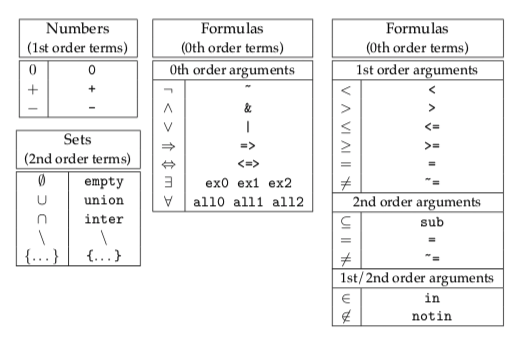
\includegraphics[width=\textwidth]{images/mona-syntax}
	\caption{The essential \MONA syntax.}
	\label{fig:mona-syntax}
\end{figure}
As we can see from that Figure, there are also quantifiers and all usual logical connectives (i.e. those used in \FOL). In addition, since we would like to write \FOL on \textit{finite linearly ordered domains}, we should enable the \mls mode specifying \texttt{m2l-str;} at the beginning of the \MONA program. Actually, \texttt{m2l-str;} is a shortcut for:
\begin{lstlisting}[style=Mona, escapechar = £]
ws1s;£\label{line:ws1s-def}£
var2 $ where ~ex1 p where true: p notin $ & p+1 in $;£\label{line:restriction}£
allpos $;£\label{line:allpos-def}£
defaultwhere1(p) = p in $;£\label{line:defaultwhere1}£
defaultwhere2(P) = P sub $;£\label{line:defaultwhere2}£
\end{lstlisting}
At the first line, it is declared the intent to use exclusively \wsos. Then, at line \ref{line:restriction}, there is the declaration of a second-order variable \texttt{\$} ensuring it to always have the value $\{0,\dots, n-1\}$ for some $n$. Likewise, it is needed the declaration at line \ref{line:allpos-def} to bound the domain of interest. Lastly, at lines \ref{line:defaultwhere1} and \ref{line:defaultwhere2}, the program restrict all first- and second-order variables to \texttt{\$}.

At this point, since we have illustrated all the necessary stuff for the translation, we are able to give the \FOL-to-\MONA encoding with some examples.

To begin with, all usual logic operators can be encoded following the table in Figure \ref{fig:mona-syntax}. Secondly, to encode the \suc and \pre monadic predicates respectively defined in Equations \ref{monadic-predicates} and \ref{prev-predicate} we use the successor and predecessor built-in operators as follows:
\begin{align*}
\suc(x,y) \doteq \texttt{y=x+1}\\
\pre(x,y) \doteq \texttt{y=x-1}
\end{align*}
Additionally, the two constants $0$ and $\last$ already defined in \ref{monadic-predicates} are encoded as \texttt{0} and \texttt{max(\$)}, respectively.
Thirdly, to express existential and universal quantifiers we use the corresponding syntax as follows:
\begin{align*}
\exists p. \doteq \texttt{ex1 p:}\\
\forall p. \doteq \texttt{all1 p:}
\end{align*}
Then, we can express first-order predicates symbols with set containment. For instance, if we have $A(x)$, before we must declare it as \texttt{var2 A;} and, then, encode it as \texttt{x in A}, whereas its negation ($\lnot A(x)$) would be \texttt{x notin A}. Finally, $\true$ and $\false$ remain the same.
In the following, we give some examples.
\begin{example}
\FOL-to-\MONA encoding examples:\\
\begin{itemize}
\item Suppose we have the \LTLf formula $\Diamond G$, its translation to \FOL according to Definition \ref{def:ltlf-to-fol} is:
\begin{equation}\label{eq:fol-eg}
\exists y. 0 \le y \le \last \lAND G(y)
\end{equation}
(we have not included the last part $\forall z. 0 \le z < y \Rightarrow \true$ since it is trivially $\true$).
The \MONA program corresponding to the formula in \ref{eq:fol-eg} is the following:
\begin{lstlisting}[style=mona]
m2l-str;
var2 G;
ex1 y: 0<=y & y<=max($) & y in G;
\end{lstlisting}

\item Suppose we have the \LTLf formula $\Box G$, its translation to \FOL according to Definition \ref{def:ltlf-to-fol} is:
\begin{equation}\label{eq:fol-gg}
\lnot (\exists y. 0 \le y \le \last \lAND \lnot G(y))
\end{equation}
The \MONA program corresponding to the formula in \ref{eq:fol-gg} is the following:
\begin{lstlisting}[style=mona]
m2l-str;
var2 G;
~(ex1 y: 0<=y & y<=max($) & y notin G);
\end{lstlisting}

\item Suppose we have the \PLTL formula $A \Since B)$, its translation to \FOL according to Definition \ref{def:pltl-to-fol} is:
\begin{equation}\label{eq:fol-asb}
\exists y. 0 \le y \le \last \lAND B(y) \lAND \forall z. y < z \le \last \Rightarrow A(z)
\end{equation}
The \MONA program corresponding to the formula in \ref{eq:fol-asb} is the following:
\begin{lstlisting}[style=mona]
m2l-str;
var2 A,B;
(ex1 y: 0<=y & y<=max($) & y in B & (all1 z: y<z & z<=max($) => z in A));
\end{lstlisting}
\end{itemize}
\end{example}
\section{Summary}
In this chapter, we have illustrated the theoretical framework, consisted of \LTL, \LTLf and \PLTL formalisms, underlying the thesis. These formal languages have been described focusing the attention on their syntax, semantics and interesting properties. Besides, we have talked about the theory behind the translation procedure of \LTLf and \PLTL formulas to \DFAs. Finally, we have presented the \MONA tool explaining in details the encoding process starting from an \LTLf/\PLTL formula to a \MONA program passing through a \FOL translation.